\documentclass[a4paper,11pt]{article}
\usepackage[utf8]{inputenc} 
\usepackage{a4wide,url,ngerman,graphicx}

\parindent0pt
\parskip3pt
\setcounter{tocdepth}{2}

\title{Partizipatorisches Virtuelles Museum\\[.6em] Entwurfsbeschreibung der
  Plattform}
\date{Version vom 18. Februar 2016}
\author{Sebastian Günther, Alexander Lieder, Hans-Gert Gräbe}

\begin{document}
\maketitle
%\tableofcontents
 
\section{Allgemein}
 
Das \emph{Partizipatorische Virtuelle Museum} (PVM) ist als digitales
Online-Museum konzipiert, in dem sich die Besucher mit Gegenständen aller Art
künstlerisch auseinandersetzen sollen. Dazu soll auf Basis von Wordpress in
Kombination mit einer eigenen Plugin-Suite und ausgewählten
Drittanbieter-Plugins in mehreren Iterationsstufen eine möglichst robuste
Lösung entwickelt werden, die moderne Designansätze wie \emph{responsive
  Design} umsetzt und auch in Zukunft Spielraum für Erweiterungen lässt.
Zusätzlich soll damit der Bedienkomfort der Seite erhöht und der
Wartungsaufwand minimiert werden.

\section{Produktübersicht}

\subsection{Prinzipielle Architektur-Entscheidungen}
 
Basis der Plattform ist eine Wordpress-Single-Site-Installation, deren Look
and Feel durch Auswahl und nachfolgende Anpassung eines geeigneten WP-Themes
für den Anwendungszweck gestaltet wird.  Zur Trennung von Layout und
Funktionalität werden eigene Plugins entwickelt, in dem die PVM-spezifischen
funktionalen Aspekte gekapselt sind. Für Stellen, wo eine Verzahnung von
Funktion und Layout erforderlich ist (etwas Such- oder Übersichtsseiten), wird
ein Child-Theme entwickelt, das auf einem \emph{leistungsfähigen Basistheme}
aufsetzt.

Mit Blick auf die Wartbarkeit und Erweiterbarkeit der Plattform sollen für
weitere abgrenzbare Aufgabenbereiche sorgfältig ausgewählte Open Source
WP-Standardplugins zum Einsatz kommen, so dass ein unabhängiges
Plugin-Upgrade möglich ist. 

\subsection{Auswahl des Basisthemes}

Als Basistheme wurde auf der Basis der Vorarbeiten der Design-Gruppe das Theme
\emph{Esteem} ausgewählt.  Auf der
Beschreibungsseite\footnote{\url{https://wordpress.org/themes/esteem/}} heißt
es:
\begin{quote}
  Esteem is a clean multipurpose responsive WordPress theme designed to fit
  business, portfolio, blogging or any type of site. The theme supports custom
  header, custom background, custom widgets, page templates and has built in
  options panel to configure primary color, site logo, slider, sidebar layout
  and 3 blog layout. It's also fully compatible with popular plugins like
  contact Form 7, WP PageNavi and Breadcrumb Navxt and is translation
  ready. 
\end{quote}
Damit sind wesentliche Grundanforderungen der Plattform bereits abgedeckt.
Weiter unterstützt das Theme Kachel-Designs, die im Plattformdesign verwendet
werden sollen. 

\subsection{Workflow aus Nutzersicht}

\begin{quote}\bf
  Die folgenden Ausführungen sind aus der Entwurfsbeschreibung des Prototyps
  übernommen, der im SWT-Praktikum erstellt wurde, und müssen noch weiter
  angepasst werden.
\end{quote}
  
Als Besucher erreicht man die Site im Regelfall über die Startseite. Dort kann
man neben News auch über verschiedene Auf"|listungen zu Objekten aus dem
Museum gelangen. Als nicht angemeldeter Betrachter hat man Zugriff auf die
Filterfunktion, mit deren Hilfe man die Ausstellungsstücke nach bestimmten
Merkmalen durchsuchen und sortieren kann. Außerdem kann man auf den einzelnen
Betrachtungsseiten die jeweiligen Ausstellungsstücke ansehen. Weitere
zugängliche Funktionen sind die Registrierung, Anmeldung sowie Impressum- und
Kontaktseiten.
 
Über die Registrierung kann ein Besucher durch Angabe weniger Daten ein
Benutzerprofil auf der Seite erstellen. Angemeldete Benutzer (nachfolgend als
“User” bezeichnet) können weitere Funktionen der Plattform nutzen. Jegliche
Partizipation an dem virtuellen Museum setzt ein Benutzerprofil voraus.

\section{Grundsätzliche Struktur- und Entwurfsprinzipien}
 
Dieses Projekt basiert auf Wordpress. Zur Realisierung der benötigten Features
soll, sofern möglich und angemessen, auf die native Wordpress-Funktionalität
und auf Community-Plugins zurückgegriffen werden. Alle weiteren Features
werden in Form von eigenen Erweiterungen umgesetzt. Diese Erweiterungen werden
im PVM-spezifischen Plugins zusammengefasst.
 
Aus Übersichtlichkeitsgründen und um die Updatefähigkeit von Wordpress zu
wahren benutzt PVMkit ein eigenes Datenmodell, das die Wordpressdatenbank um
mehrere Tabellen erweitert.
 
PVMkit hat eine eigene Verzeichnis- bzw. Dateistruktur. Im Hauptverzeichnis
\texttt{pvmkit} befinden sich die Dateien \texttt{pvmkit.php},
\texttt{pvmkit\_functions.php} und \texttt{pvmkit\_install.php} sowie die
Ordner \texttt{admin} und \texttt{includes}. Der \texttt{admin}-Ordner enthält
Funktionen und Erweiterungen, die gänzlich oder zum überwiegenden Teil ins
Backend einzuordnen sind, während im \texttt{includes}-Ordner die
Frontend-Funktionalität ihren Platz findet.
 
Logische Funktionen sind innerhalb dieser Ordner in separaten Dateien
untergebracht. So enthält beispielsweise die Datei \texttt{pvmkit\_viewer.php}
(includes) den Code, der für das Anzeigen von Werken im Frontend
verantwortlich ist. Die unter Punkt 4 genannten Pakete sind
u.U. dateiübergreifend, d.h.\ ein Paket kann mehrere Dateien umfassen.
\begin{itemize}
\item Die Datei \texttt{pvmkit.php} dient als Container, über den die
  Funktionalitäten aus dem Verzeichnissen \texttt{admin} und \texttt{includes}
  eingebunden werden.
\item \texttt{pvmkit\_functions.php} enthält Funktionen, die keiner logischen
  Funktion konkret zugeordnet werden konnten bzw. die in mehreren Dateien
  inkludiert werden.  
\item \texttt{pvmkit\_install.php} ist für Anweisungen zur erstmaligen
  Installation des Plugins (Anlegen von Benutzerrollen, Erstellen von
  Datenbanktabellen) gedacht.
\end{itemize}
Das Darstellen von Werken und Projekten im Frontend wird über Shortcodes
realisiert.  Dazu wird ein Wordpress-Post erstellt, der einen Shortcode mit
der ID des jeweiligen Werks bzw. Projekts enthält.
 
Eingebundene Community-Plugins sollten nicht verändert werden. Falls eine
Änderung im Code eines solchen Plugins unvermeidbar ist, wird diese als Patch
eingespielt.
 
\section{Struktur- und Entwurfsprinzipien einzelner Pakete}
 
\subsection{Erstellen und Verwalten von Werken und Projekten}
 
Dateien: 
\begin{itemize}\itemsep0pt\tt
\item pvmkit/admin/pvmkit\_composition\_manager\_user.php 
\item pvmkit/admin/pvmkit\_project\_manager.php
\item pvmkit/admin/pvmkit\_projects.php
\item pvmkit/admin/pvmkit\_publish\_compositions.php
\end{itemize}

Die Funktionalität des Einsendens neuer Werke durch Benutzer wird von einem
Backend-Modul bereitgestellt. Der Einsendeprozess ist modular aufgebaut.
Zunächst muss das Werk vom Benutzer durch das Hinzufügen der
Einzelbestandteile (Titel, Text, Titelbild etc.)  zusammengestellt werden.
Dafür ist die Datei \texttt{pvmkit\_composition\_manager\_user.php}
verantwortlich. Darin werden etliche Formulare für diesen Zweck
bereitgestellt.  Hochgeladene Bilder werden automatisch in drei Größen (small
-- 50$\times$50, medium -- 200$\times$200, large -- 600$\times$Variabel)
transformiert und unter \texttt{uploads/pvmkit} abgelegt. Der Dateiname wird
automatisch erzeugt und setzt sich aus der \texttt{element\_id} des Bildes und
dessen Größenbezeichnung zusammen, z.B.  \texttt{81\_medium.jpg}.
 
Alternativ können Objekte (Bilder, Texte) auch im Frontend von anderen Werken
durch einen Klick auf Bild verwenden bzw.  Text verwenden übernommen werden.
Bei Bildern wird lediglich die \texttt{element\_id} mit dem neuen Werk
verknüpft. Bei Texten hingegen wird der Text als neues Objekt kopiert, um
ungewollte Modifikationen zu vermeiden.
 
Ist das Werk fertig, wird sein Status zu 3 geändert. Damit ist das Werk zur
Moderation freigegeben. Diese Aufgabe übernimmt die Datei
\texttt{pvmkit\_publish\_compositions.php}.  Die dortige Freischaltung setzt
den Status auf 7. Es wird ein Wordpress-Post mit dem Shortcode
\texttt{[pvmkit\_viewer id=xx]} erstellt, woben \texttt{xx} für die ID des
Werks steht. Das Werk ist damit veröffentlicht und wird im Frontend angezeigt.
 
\texttt{pvmkit\_projects.php} stellt Funktionen zur globalen Verwaltung von
Projekten und Projektleitern bereit, während
\texttt{pvmkit\_project\_manager.php} Funktionen zur Verwaltung eigener
Projekte enthält.
 
\subsection{Darstellung von Werken und Projekten im Frontend sowie die
  Verwaltung gemeldeter Verstöße}
 
Dateien:  
\begin{itemize}\itemsep0pt \tt 
\item pvmkit/includes/pvmkit\_viewer.php
\item pvmkit/includes/pvmkit\_view\_project.php
\item pvmkit/includes/pvmkit\_list\_widget.php
\item pvmkit/includes/pvmkit\_filter.php
\item pvmkit/admin/pvmkit\_report\_manager.php
\end{itemize}
Werke werden mittels des Shortcodes \texttt{[pvmkit\_viewer id=xx]}
veröffentlicht, für das Abrufen der Daten aus der Datenbank ist
\texttt{pvmkit\_viewer.php} verantwortlich. Für Projekte wird der Shortcode
\texttt{[pvmkit\_view\_project pid=xx]} verwendet, die zuständige Datei ist
\texttt{pvmkit\_view\_project.php}.
 
\texttt{pvmkit\_list\_widget.php} erstellt eine Liste der neuesten
veröffentlichten Werke, indem die Datensätze in der \texttt{pvm\_compositions}
Tabelle nach dem Erstellungsdatum sortiert und die ersten 10 Einträge
ausgelesen werden.
 
Das Formular zum Melden eines Verstoßes wird in \texttt{pvmkit\_viewer.php}
erzeugt und ist zu"|nächst mittels des CSS-Tags \texttt{display:none}
verborgen, bis der Link „Einen Verstoß melden” angeklickt wird.  Dies wird in
der Tabelle \texttt{pvm\_reported\_compositions} gespeichert.
 
Gemeldete Verstöße werden über \texttt{pvmkit\_report\_manager.php} im Backend
unter dem Punkt „Gemeldete Werke” gelistet und verwaltet.
 
\subsection{Benutzerregistrierung und Authentifizierung, Benutzerprofil
  anzeigen und bearbeiten}
 
Dateien und Ordner:  
\begin{itemize}\itemsep0pt\tt
\item wp-members
\item really-simple-captcha
\item pvmkit/includes/pvmkit\_list.php
\item pvmkit/includes/pvm\_user\_profile.php
\end{itemize}
 
Für die Benutzerregistrierung und Authentifizierung sowie zur Verwaltung der
Benutzerprofile kommt das Plugin \texttt{wp-members} zum Einsatz. Es bietet
die Basisfunktionalität, die man von anderen Community-basierten Portalen
gewohnt ist (Registrierungs- und Loginformular, Aktivierung des Accounts durch
eine Bestätigungsemail, „Password vergessen”-Funktion etc.)  und kann ohne
Veränderung des Codes aus dem Backend konfiguriert werden.
 
Zur Verhinderung automatischer Registrierungen durch Bots wird
\texttt{wp-members} durch das Plug"|in \texttt{really-simple-captcha}
erweitert, das speziell auf \texttt{wp-members} zugeschnitten ist.
 
\texttt{wp-members} nutzt das Datenmodell von Wordpress und speichert
Nutzerdaten in den Tabellen \texttt{users} sowie \texttt{usermeta}.
 
Das Benutzerprofil wird durch \texttt{pvmkit\_list.php} in Verbindung mit
\texttt{pvm\_user\_profile.php} um eine Liste der von dem jeweiligen Benutzer
veröffentlichten Werke erweitert. 
\begin{itemize}
\item \texttt{pvmkit\_list.php} stellt dabei die Liste mittels eines
  Shortcodes (\texttt{[pvmkit\_list]}) zur Verfügung und
\item \texttt{pvm\_user\_profile.php} inkludiert diesen Shortcode.  
\end{itemize}
Durch die Trennung dieser beiden Aufgaben ist es möglich, die Liste auch an
anderen Stellen des PVM durch den Shortcode anzuzeigen.
 
\subsection{Statistiken}
 
Dateien:  
\begin{itemize}\itemsep0pt\tt
\item pvmkit/admin/pvmkit\_statistics.php 
\end{itemize}

\texttt{pvmkit\_statistics.php} erzeugt unterschiedliche Statistiken zum PVM
(Gesamtzahl der Werke, beliebtestes Werk, aktivster Benutzer etc.) im Backend
unter dem Menüeintrag „Statistiken”.
 
\subsection{Social-Media Buttons (Shariff)}
 
Auf verschiedenen Seiten sollen (nicht kontextsensitive) Social Media Buttons
für Aktionen wie Teilen und „Liken” angeboten werden. Damit sollen alle großen
Netzwerke abgedeckt werden.  Die Beachtung von Datenschutz spielt eine große
Rolle.
 
Unter den wenigen datenschutzkonformen Lösungen wird Shariff noch regelmäßig
mit Updates versorgt und kann separat aktualisiert werden. Es kann sowohl als
Widget in die Sidebar als auch als Shortcode eingebunden werden, womit die
nötige Flexibilität gegeben ist. Shariff unterstützt alle größeren sozialen
Netzwerke.

\subsection{Theme} 
 
Dateien und Ordner:  
\begin{itemize}\itemsep0pt\tt
\item twentyfifteen-pvmkit/
\item twentyfifteen-pvmkit/author.php
\item twentyfifteen-pvmkit/content.php
\item twentyfifteen-pvmkit/functions.php
\item twentyfifteen-pvmkit/index.php
\item twentyfifteen-pvmkit/single-project.php
\item twentyfifteen-pvmkit/single-search.php
\item twentyfifteen-pvmkit/style.css
\end{itemize}
 
Als Theme wurde „Twenty Fifteen“ ausgewählt, da es sich durch Einfachheit im
Design und eine unproblematische Modifizierbarkeit auszeichnet. Für
projektspezifische Änderungen des Themes wurde unter
\texttt{twentyfifteen-pvmkit} ein Child-Theme angelegt.
 
\texttt{index.php} und \texttt{content.php} folgen den Wordpress Standards und
stellen eine Liste sowie die Einzelbetrachtungsseite der Posts zur Verfügung.
 
In \texttt{single-search.php} und \texttt{single-project.php} sind, wie die
Namen bereits verraten, Funktionen für den Suchvorgang sowie die Darstellung
der Projektseiten untergebracht.
 
\paragraph{Erweiterungsmöglichkeiten:}
Grundlegende Veränderungen am Layout sollten innerhalb des Child-Themes
geschehen, Designanpassungen etwa in der Datei \texttt{style.css} im
Verzeichnis \texttt{twentyfifteen-pvmkit} vorgenommen werden.
 
\section{Datenmodell}
 
Das Standard-Wordpress-Datenmodell wird nicht verändert, um eine reibungslose
Funktion und Updatefähigkeit des Grundsystems sicherzustellen. Das
PVM-Datenmodell ist deshalb konzipiert als Erweiterung des WP-Datenmodells um
PVM-spezifische Begrifflichkeiten, die über drei Bindings -- (1) an die
Tabellenstruktur der SQL-Datenbank, (2) an einen eigenen Upload-Bereich im
Dateisystem des Webservers und (3) an die CSS-Struktur des verwendeten
WP-Basisthemes -- die entsprechenden WP-Datenrepräsentationen erweitert. 

\begin{figure}[t]
  \begin{center}
    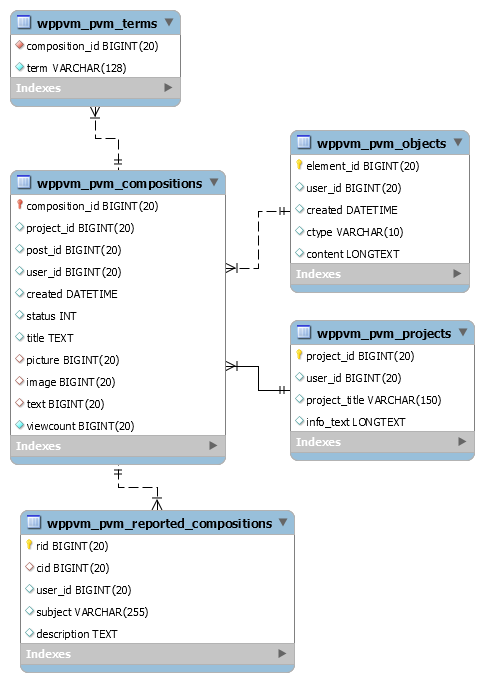
\includegraphics[width=.6\textwidth]{DB-Tabellen.png}
    \caption{Die fünf PVMkit-Tabellen mit Wordpress-Präfix \texttt{wppvm\_}}
  \end{center}
\end{figure}

Die Erweiterung (1) der Datenbank erfolgt durch (zunächst) vier Tabellen,
welche durch das Präfix \texttt{pvm\_} gekennzeichnet sind:
\begin{itemize}
\item \texttt{pvm\_compositions}: Ein Datensatz dieser Tabelle repräsentiert
  ein Werk, welches von einem User eingesendet wurde.
\item \texttt{pvm\_objects}: Ein Datensatz dieser Tabelle stellt ein Element
  eines Werkes da, also ein Text oder Bild. Dieses Element kann in mehreren
  Werken Verwendung finden.
\item \texttt{pvm\_projects}: Ein Datensatz dieser Tabelle repräsentiert ein
  Projekt, welches von einem User initiiert wurde. Werke können maximal einem
  Projekt zugeordnet werden.
\item \texttt{pvm\_terms}: Ein Datensatz dieser Tabelle stellt die Zuordnung
  des Tags („term”) zu einem Werk („composition\_id” aus pvm\_compositions)
  dar. Dabei handelt es sich technisch gesehen um eine $m:n$-Beziehung, welche
  allerdings bewusst nicht aufgelöst wurde. Im momentanen Projekt wäre der zu
  erwartende Mehraufwand in der Verwaltung ungünstiger als die zu erwartenden
  Kollisionen/Redundanz.
\item \texttt{pvm\_reported\_compositions}: Ein Datensatz dieser Tabelle
  stellt einen gemeldeten Verstoß dar.  Die Zuordnung erfolgt über einen
  Fremdschlüssel auf die composition\_id des gemeldeten Werks. Ein Betreff
  bzw. eine Kurzbeschreibung des Verstoßes (subject) ist obligatorisch, die
  detaillierte Beschreibung (description) ist fakultativ.
\end{itemize}
Die wesentliche Datenbasis stellen die Tabellen \texttt{pvm\_compositions}
(Werke) und \texttt{pvm\_objects} (Elemente) dar. Einem Werk können über die
Attribute \texttt{text}, \texttt{image} und \texttt{picture} aus
\texttt{pvm\_compositions} bis zu drei Elemente (aus \texttt{pvm\_objects})
zugeordnet werden. Ist eines dieser Attribute nicht belegt, wird es auf NULL
gesetzt. Als Untergrenze für ein Werk sind minimal zwei Elemente vorgesehen,
was allerdings im Datenbanksystem nicht als Integritätsbedingung festgelegt
ist. Damit ist es beispielsweise später möglich, Teile eines Werkes zu löschen
oder zur Überarbeitung an den Nutzer zu melden.
 
Die Tabelle \texttt{pvm\_compositions} erlaubt außerdem für weitere Attribute
den NULL-Wert:
\begin{itemize}
\item \texttt{project\_id}: NULL bedeuted in diesem Fall, dass das Werk nicht
  explizit einem Projekt zugeordnet ist. Es impliziert im Gegenzug, dass
  Aufgaben wie die Tagauswahl oder Zulassung zu einem Projekt nicht an einen
  Projektleiter aus der Menge der User delegiert werden kann.
 
\item \texttt{post\_id}: Dieses Attribut bezieht sich auf das ID-Attribut der
  posts-Tabelle von Wordpress. Wenn es NULL ist, ist der Post noch nicht
  veröffentlich oder gelöscht worden. Wenn es einen numerischen Wert besitzt,
  ist es der Post, unter dem das Werk in Wordpress veröffentlicht wurde. Eine
  eindeutige Information über den Status des Werkes ist über das Feld status
  zu beziehen (7 und größer: veröffentlicht).
\end{itemize}
Die in einigen Tabellen angegebenen \texttt{user\_id}-Attribute beziehen sich
auf die Wordpress-User-ID (Feld ID in der \texttt{users}-Tabelle von
Wordpress).
 
Die Datentypen orientieren sich im Regelfall an den Werten, die auch Wordpress
in seinem Datenmodell verwendet. Für IDs wird \texttt{BIGINT(20)} verwendet
und Zeitpunkte als \texttt{DATETIME}\footnote{Dies ist für
  \texttt{CURRENTTIME} problematisch, da hier der Datentyp \texttt{TIMESTAMP}
  erwartet wird und die Umrechnung nicht immer automatisch funktioniert.\par 
  Siehe etwa \url{http://phpforum.de/forum/showthread.php?t=269679} für
  weitere Informationen.}.
 
Die Rückzuordnung eines Posts zum Werk ist auf semantischer Ebene gegeben
durch den Parameter im Shortcode des \texttt{post\_content}-Attributs. Durch
die Einbindung als Shortcode wird eine Datenunabhängigkeit erreicht, sodass
durch Austausch des Viewers beispielsweise das Aussehen komplett verändert
werden kann.

\paragraph{Merkmale:}
Merkmalsausprägung und Typ sind in der DB-Tabelle \texttt{pvmkit\_properties}
aufgelistet, der Typ nur als Textfeld, da verschiedene Merkmale verschieden
visualisiert werden, was (derzeit) hart im Frontend zu kodieren ist.
\texttt{pvmkit\_property\_index} enthält die Kreuzreferenzen der Merkmale der
einzelnen Werke.
 
\end{document}
